For extensions of the Higgs sector containing two Higgs doublets, the couplings of the heavy Higgs bosons to down-type fermions can be enhanced with respect to the SM for large tan$\beta$ values.  These results in increased branching fractions to $\tau$ (and $\mu$) leptons and $b$ quarks, as well as a higher cross section for Higgs boson production in association with $b$-quarks. This has motivated a variety of searches in $\tau\tau$, $bb$ and $\mu\mu$ final states at the LHC -Run1 \cite{Hmumu_ref_CMS,Hbb_ref_CMS,Aad:2014vgg,Aad:2012cfr,Aad:2011rv} with no indication of an excess over the expected SM background.


%The ATLAS collaboration the CMS collaboration have
%performed searches for neutral Higgs bosons decaying to $\tau$ leptons using proton--proton collision data collected at a centre-of-mass energy of 13 TeV in 2015\cite{ATLAS-CONF-2015-061,CMS:2016pkt}.
The Run-2 search for neutral Higgs bosons decaying to $\tau$ leptons  is performed in three channels by the  ATLAS collaboration\cite{ATLAS-CONF-2015-061}: the $\tau_{e}$$\tau_{\rm had}$ channel where one $\tau$ decays leptonically to an electron and neutrinos and the
other hadronically (to hadrons and a neutrino),  
the $\tau_{\rm \mu}$$\tau_{\rm had}$ channel where the leptonically decaying $\tau$ produces a muon and neutrinos,  and  the  $\tau_{\rm had}$$\tau_{\rm had}$ channel where both $\tau$ leptons decay hadronically. 
In addition to the previous three channels, the CMS collaboration extended the search in the $\tau_{e}\tau_{\mu}$ channel  in which both  $\tau$'s decay leptonically \cite{CMS:2016pkt}.
In addition, the CMS collaboration divided the events into two categories based on the number of b-tagged jets: events with  exactly zero b-tagged jets and events with at least one b-tagged jet.

\subsection{$\tau_{\rm had}$ reconstruction}
The reconstruction and the identification of hadronic decays of $\tau$ leptons are critical aspects for the searches of neutral  Higgs bosons $H/A$.
The hadronic decays of $\tau$ leptons are predominantly characterised by the presence of one or three charged particles, accompanied by a neutrino and possibly neutral pions. In ATLAS, as reported in Ref. \cite{ATL-PHYS-PUB-2015-045}, the reconstruction of the visible decay products of the hadronic decays of $\tau$ %, hereafter referred to as $\tau_{\rm had-vis}$,
starts with jets reconstructed from calorimeter clusters using the anti-kt algorithm with a radius of $\Delta R = 0.4$ \cite{Cacciari:2008gp}. The $\tau_{\rm had}$ candidate must have energy deposits in the calorimeters in the range $|\eta| < 2.5$, with the transition region between the barrel and end-cap calorimeters ($1.37 < |\eta| < 1.52$) excluded, have a transverse momentum greater than 20 GeV, one or three associated tracks and an electric charge of $\pm1$. A multivariate Boosted Decision Tree (BDT) based identification is used to reject backgrounds from jets, using shower shape and track multiplicity properties. An additional dedicated likelihood-based veto is used to reduce the number of electrons misidentified as $\tau_{\rm had}$. In the ATLAS analysis, two $\tau_{\rm had}$ identification selections are used: "loose" and "medium" with efficiencies for true $\tau_{\rm had}$ objects of about 65\% and 55\%, respectively. In CMS, hadronically decaying $\tau$ leptons are reconstructed using the hadron-plus-strips algorithm \cite{Khachatryan:2015dfa}.
The algorithm considers candidates with one charged pion and up to two neutral pions, or
three charged pions, and is seeded by a jet. The neutral pions decay rapidly into two photons,
and they are reconstructed as "strips" of electromagnetic particles, formed from energy depositions in the electromagnetic calorimeter ECAL. 
The $\tau$ decay mode is reconstructed by combining the charged hadrons with the ECAL strips. 
The $\tau_{\rm had}$ candidate must have $|\eta| < 2.3$ and a transverse momentum greater than 20 GeV for the $\tau_{e}$$\tau_{\rm had}$ and  $\tau_{\mu}$$\tau_{\rm had}$ channels, while $|\eta| < 2.1$ and $p_{\rm T}>40$ GeV for the  $\tau_{\rm had}$$\tau_{\rm had}$ channel. The $\tau_{\rm had}$ candidates that are also compatible with muons
or electrons are rejected. Jets originating from the hadronization of quarks and gluons are suppressed
by requiring the $\tau_{\rm had}$ candidate to be isolated, where the isolation variable is computed using
a multivariate (MVA) approach \cite{Khachatryan:2015dfa}. 

\subsection{The $\tau_{\rm had}\tau_{\rm had}$, $\tau_{e}\tau_{\rm had}$, $\tau_{\mu}\tau_{\rm had}$ and $\tau_{e}\tau_{\mu}$ channels}
In the $\tau_{\rm had}$$\tau_{\rm had}$ channel, multi-jet events form the dominant background, and they are estimated using a data-driven techniques by both collaborations, with a  fake-factor method in ATLAS, and with events in data with slightly looser isolation conditions compared to the the signal regions in CMS. These events are then weighted by the extrapolation factor from the nominal selection to this control region as measured in data events with $\tau_{\rm had}$ candidate having the same charge. Events from other processes with a jet misidentified
as a $\tau_{\rm had}$, such as W+jets and top-quark backgrounds, are taken from simulation and, in ATLAS,
corrected using fake rates measured from data. Events with correctly identified $\tau_{\rm had}$ are taken
from simulation, with additional derived data/MC corrections.


In the $\tau_{e}$$\tau_{\rm had}$ and $\tau_{\mu}$$\tau_{\rm had}$ channels, the background is composed by  processes involving jets misidentified as $\tau_{\rm had}$ (multi-jet, $W$+jets),  processes with electrons misidentified as a $\tau_{\rm had}$ ($Z/\gamma\rightarrow ee$), and backgrounds with a correctly identified $\tau_{\rm had}$ ($Z/\gamma\rightarrow \tau\tau$ or $t\bar{t}\rightarrow W^{+}W^{-}b\bar{b}\rightarrow l \tau_{\rm had}\nu \bar{\nu}b\bar{b}$).
To suppress the $W$+jets backgrund, a cut to reject events with transverse mass $m_{\rm T}(l,E_{\rm T}^{\rm miss})$ (where $l$ is the electron or the muon, and $E_{\rm T}^{\rm miss}$ is the missing transverse momentum) compatible with the $W$ boson are used by both the collaborations.
Backgrounds from all processes that involve jets misidentified as $\tau_{\rm had}$ are estimated simultaneously in a data-driven  method. For W+jets, the measurement is performed in a region identical to the signal region, but with reversed cut on $m_{\rm T}(l, E_{\rm T}^{\rm miss})$. The multi-jet background is measured in a region defined by inverting the isolation requirement of the electron or muon by the ATLAS collaboration, and by inverting the requirement on the relative charge of the $\tau_{\rm had}$ with respect to the electron or to the muon by the CMS collaboration.
Events with electrons misidentified as a $\tau_{\rm had}$ are suppressed by the ATLAS collaboration with a veto of events with the mass $m(\tau_{\rm had},l)$ in the Z boson mass window, $80~{\rm GeV} < m(\tau_{\rm had},l) < 110~{\rm GeV}$, while the CMS collaboration uses a veto of events containing a pair of opposite sign electrons or muons passing slightly looser identification and isolation conditions.
Backgrounds with a correctly identified $\tau_{\rm had}$ are taken from simulation, with additional derived data/MC corrections.

Finally, for the $\tau_{e}\tau_{\mu}$ channel studied by the CMS collaboration, the contribution from $W$+jets is small and taken from MC.  Events with same sign $(e,\mu)$ are used after subtracting the other backgrounds for the multi-jet estimate. All the other backgrounds are taken from simulation, with additional derived data/MC corrections.

The transverse invariant mass of the ditau candidate pair, $m_{\rm T}(\tau_{1},\tau_{2})$, is used to search for a possible
signal contribution on top of the expected backgrounds by the CMS collaboration, while ATLAS used the total transverse mass, defined as $m_{\rm T}^{tot}=\sqrt{m_{\rm T}^{2}(\tau_{1},\tau_{2})+m_{\rm T}^{2}(\tau_{1},E_{\rm T}^{\rm miss})+m_{\rm T}^{2}(\tau_{2},E_{\rm T}^{\rm miss})}$. 
The results of both collaborations show an observed event yield compatible with the expected event yield from SM processes, within uncertainties. The $m_{\rm T}(\tau_{1},\tau_{2})$ and $m_{\rm T}^{tot}$ distributions for representative signal regions are shown in Fig. \ref{fig_1Htautau}.
\begin{figure}
\centering
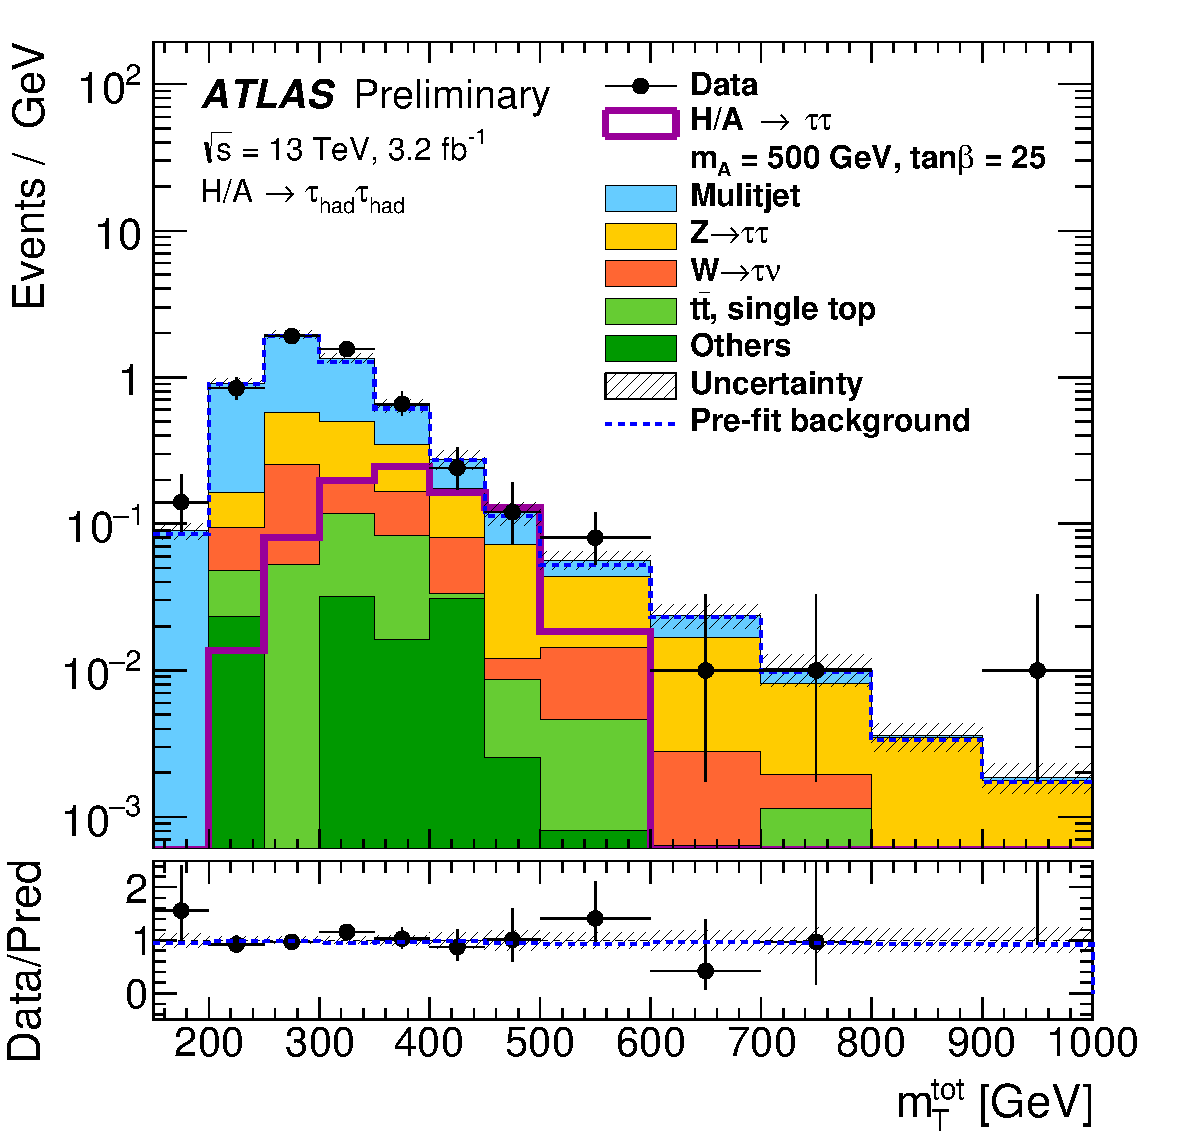
\includegraphics[width=0.48\textwidth, angle=0] {figures/fig_1Htautau_a.pdf}
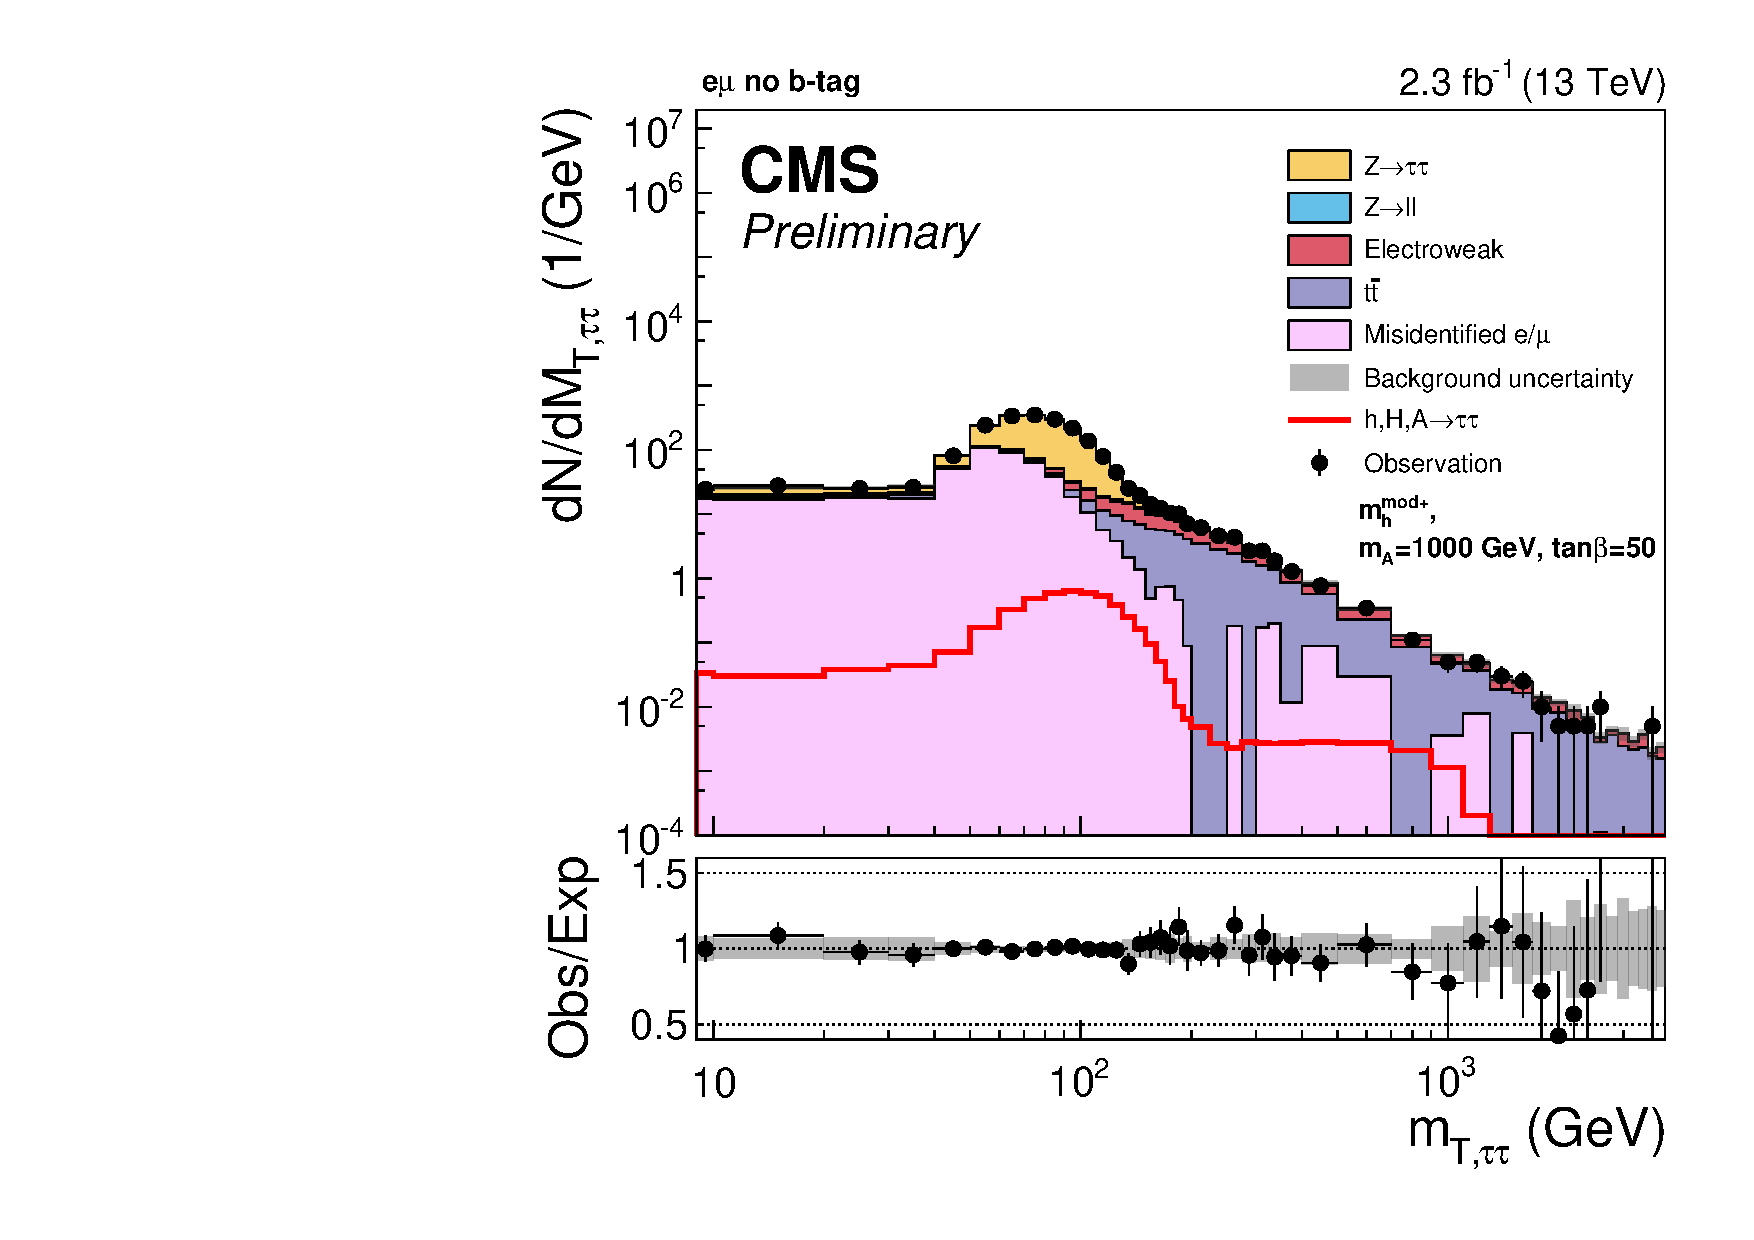
\includegraphics[width=0.48\textwidth, angle=0] {figures/fig_1Htautau_b.pdf}
\caption{ (Left) Post--fit plot of the total transverse mass distribution in f the $\tau_{\rm had}\tau_{\rm had}$ channel by the ATLAS collaboration. (Right) Post--fit plot of the transverse mass distribution in the no b--tag category of the $\tau_{e}\tau_{\mu}$ channel by the CMS collaboration.}
\label{fig_1Htautau}   
\end{figure}

\subsection{Results}
The final results are provided both as limits on the cross section times branching ratio as well
as a model-dependent limits on various MSSM benchmark models. The limits for all channels combined are shown in Fig. \ref{fig_2aHtautau} and Fig. \ref{fig_2bHtautau}
for the gluon fusion and b-associated production methods respectively, while Fig. \ref{fig_3Htautau} shows the expected and observed 95\% CL upper limits on tan$\beta$ as a function of $m_{A}$ in the MSSM $m_{h}^{mod+}$ scenario, and the comparison with the LHC Run1 results. Already with the  limited statistics recorded in 2015, the sensitivity exceeds the 8 TeV result for $m_{H} >$ 750 GeV for ATLAS and  $m_{H} >$ 350 GeV for CMS. 

\begin{figure}
\centering
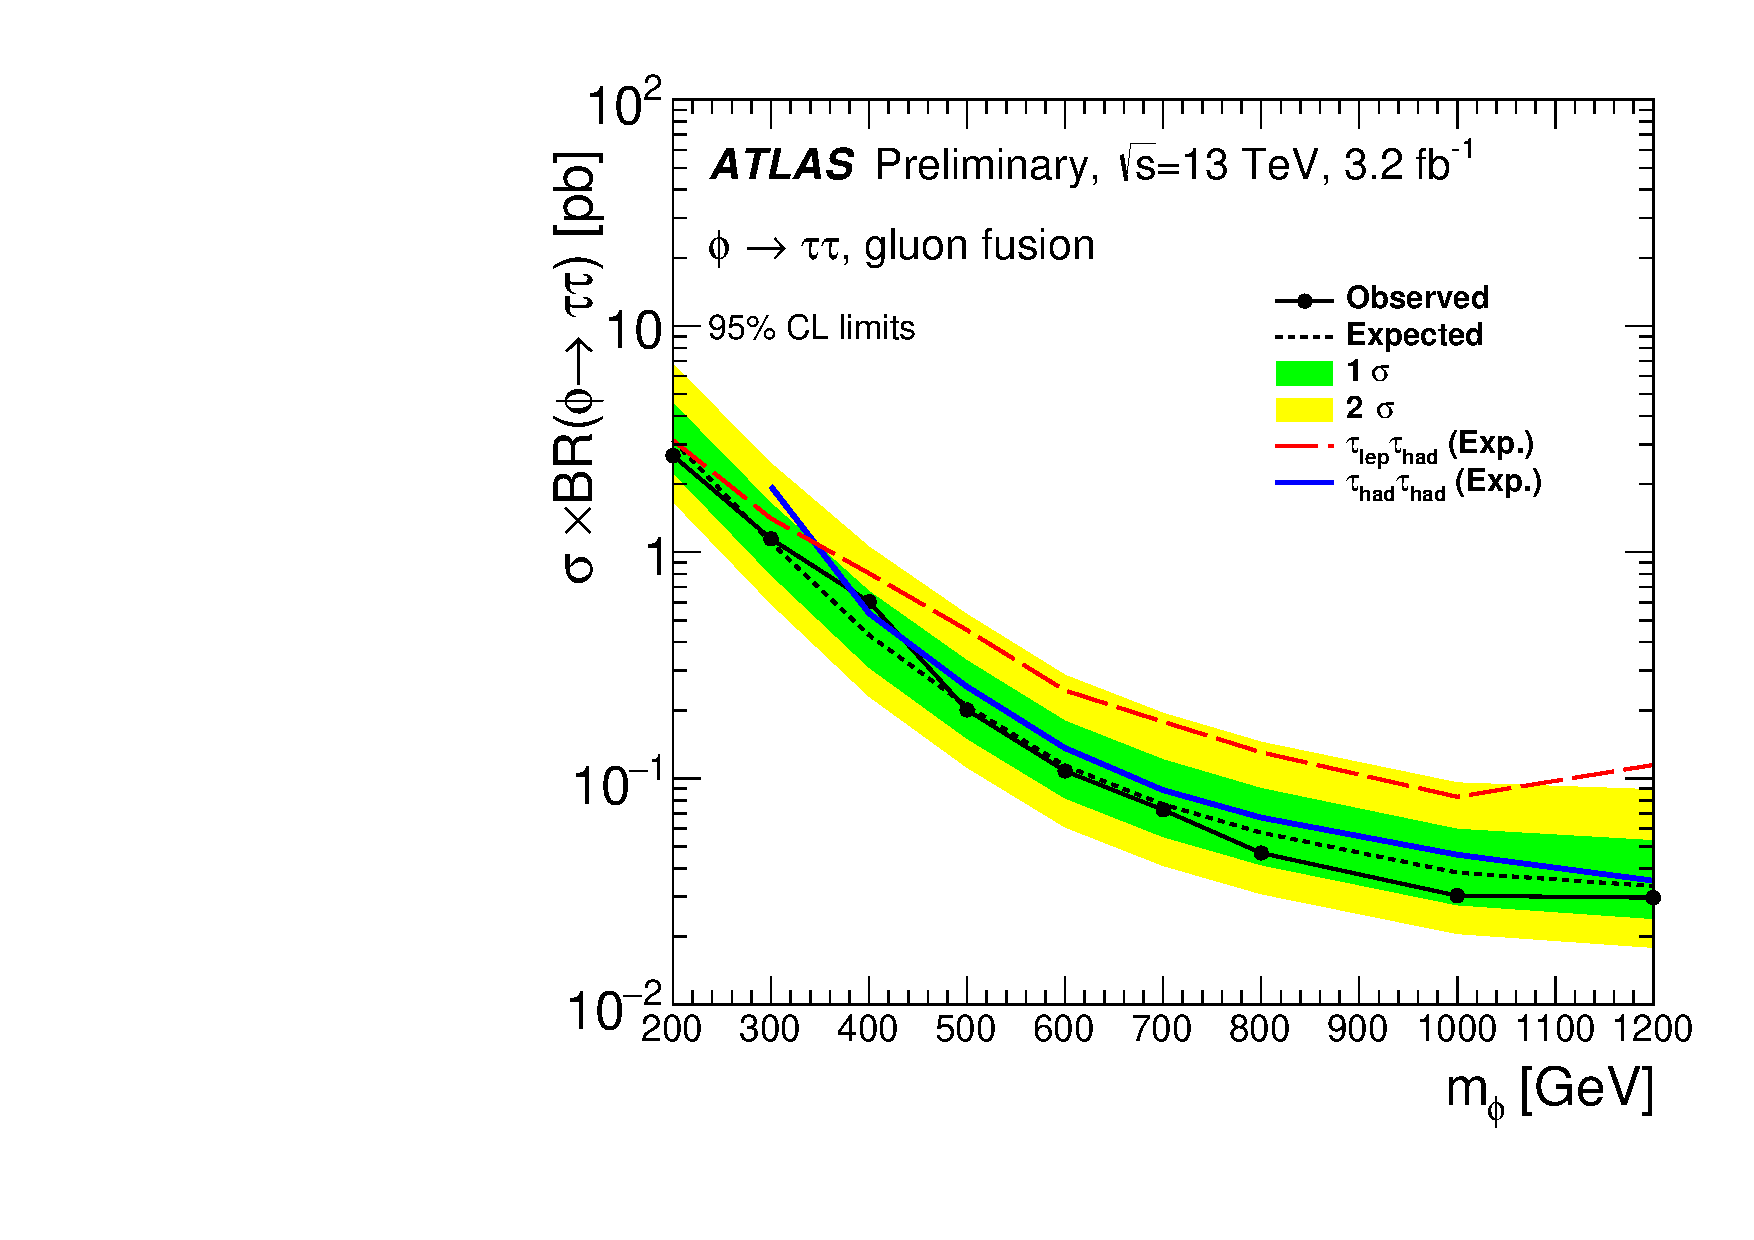
\includegraphics[width=0.48\textwidth, angle=0] {figures/fig_2Htautau_a.pdf}
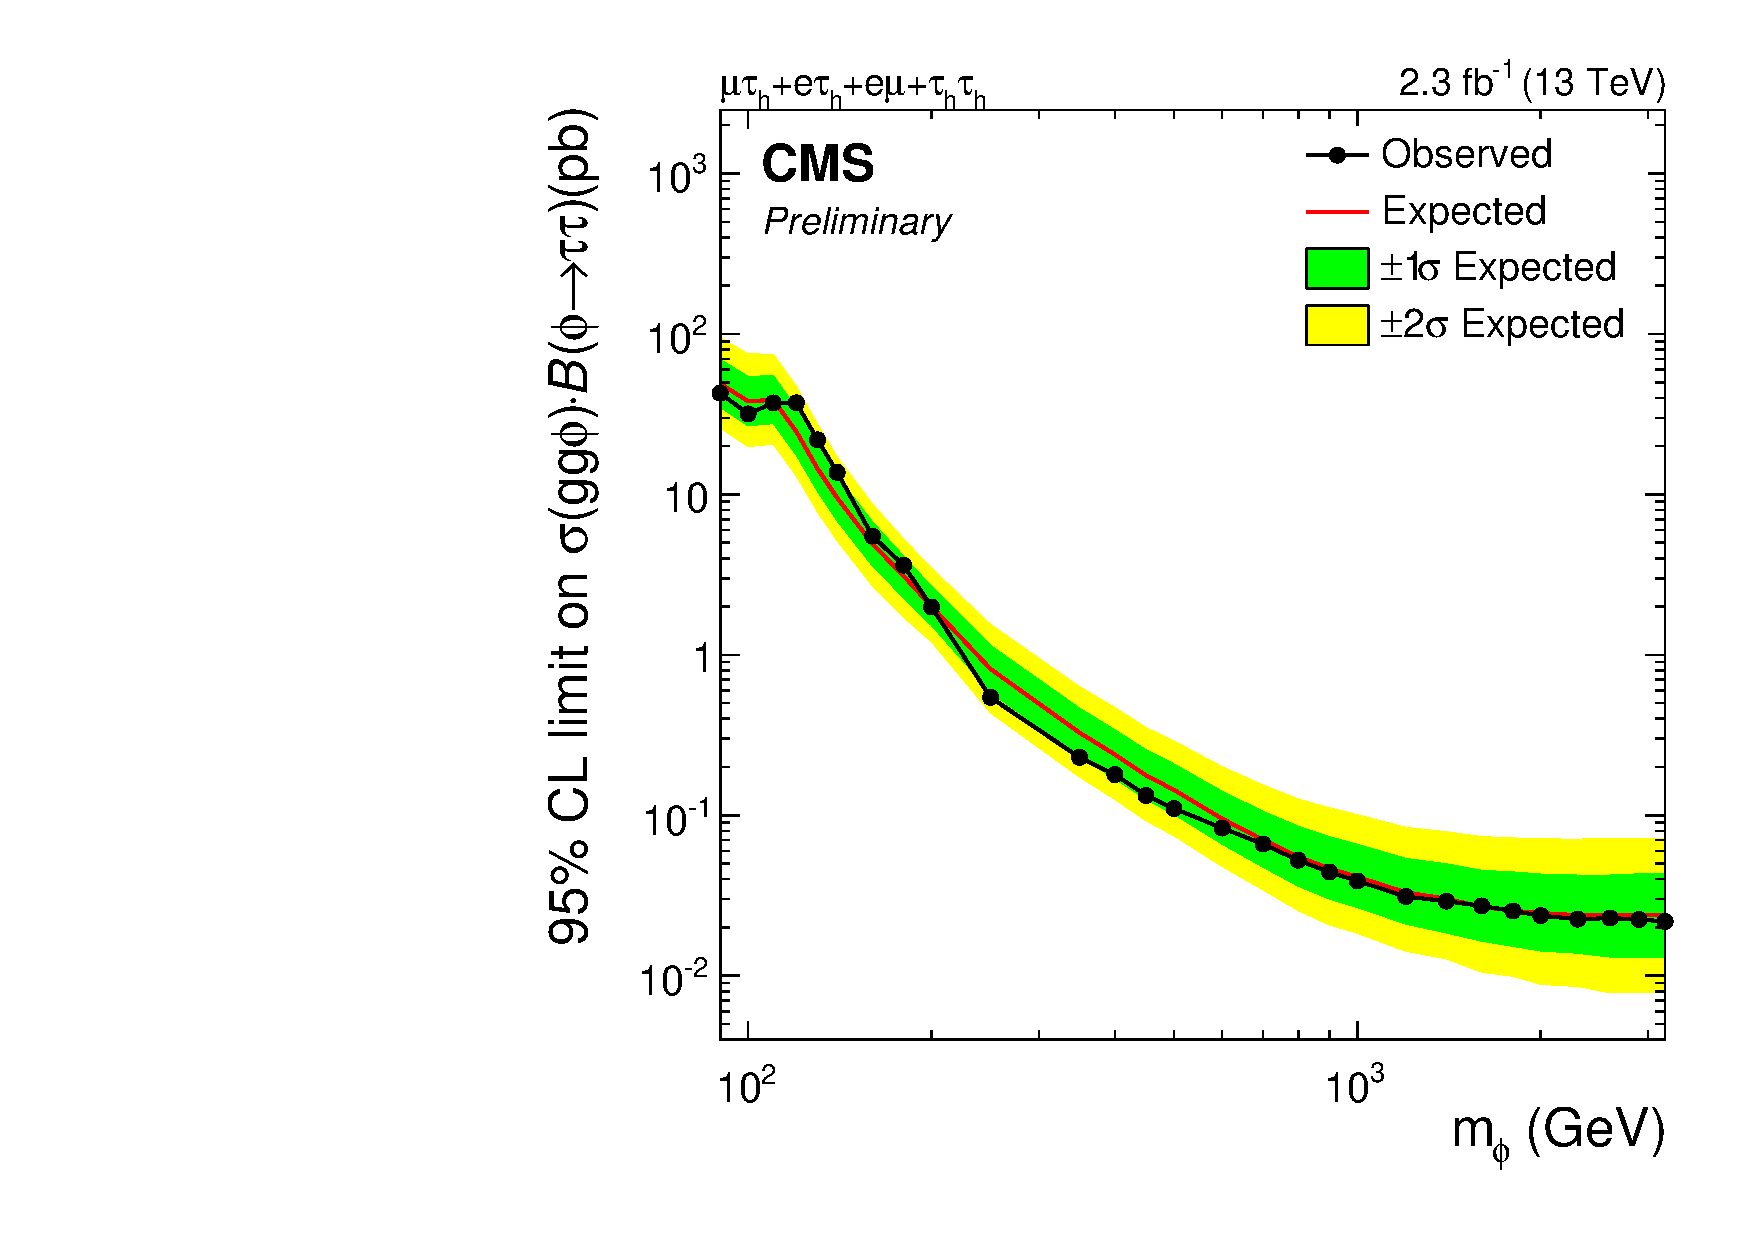
\includegraphics[width=0.48\textwidth, angle=0] {figures/fig_2Htautau_c.pdf}
\caption{ Observed and expected 95\% CL upper limits on the product of cross section and the branching fraction $\sigma(pp\rightarrow \phi) \times B(\phi\rightarrow \tau\tau)$ obtained by the ATLAS collaboration (left) and by the CMS collaboration (right) for the gluon-gluon fusion production.}
\label{fig_2aHtautau}   
\end{figure}

\begin{figure}
\centering
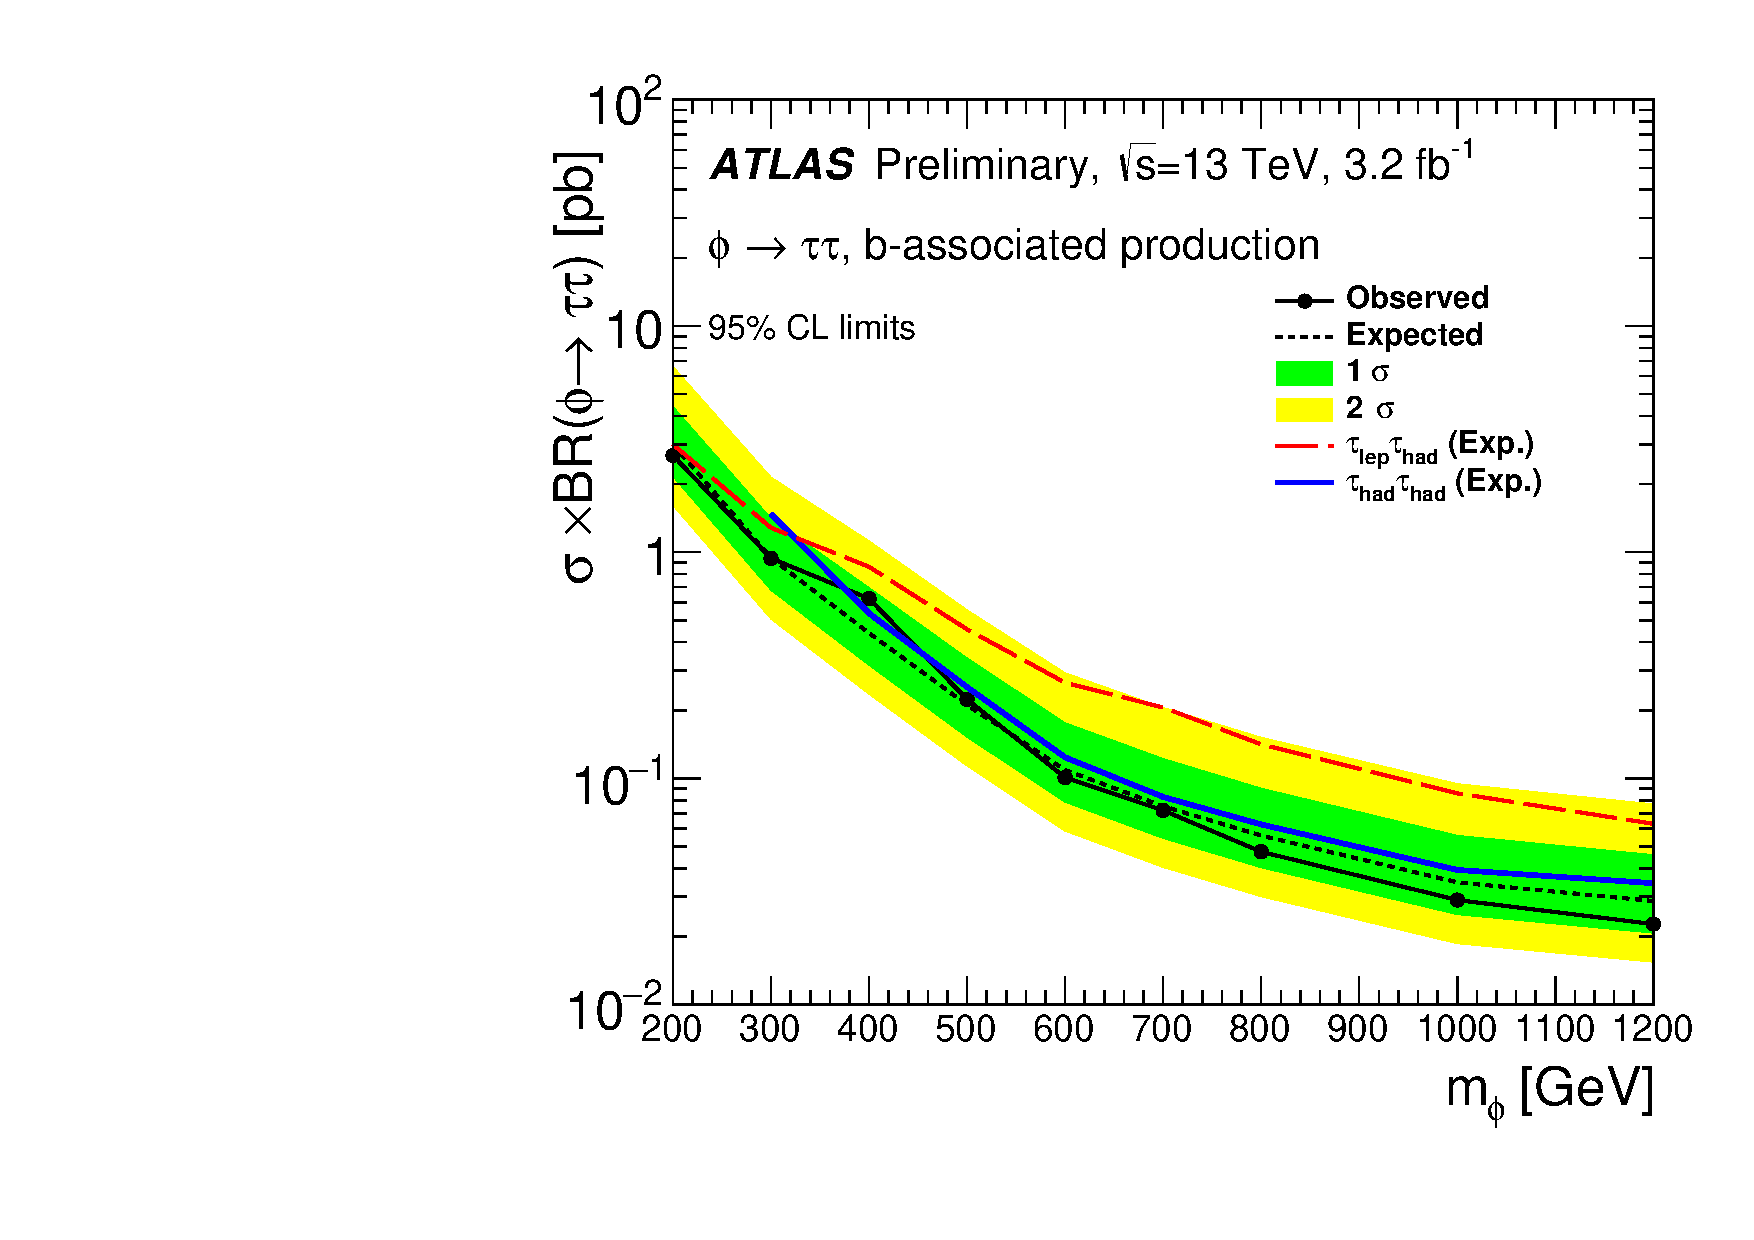
\includegraphics[width=0.48\textwidth, angle=0] {figures/fig_2Htautau_b.pdf}
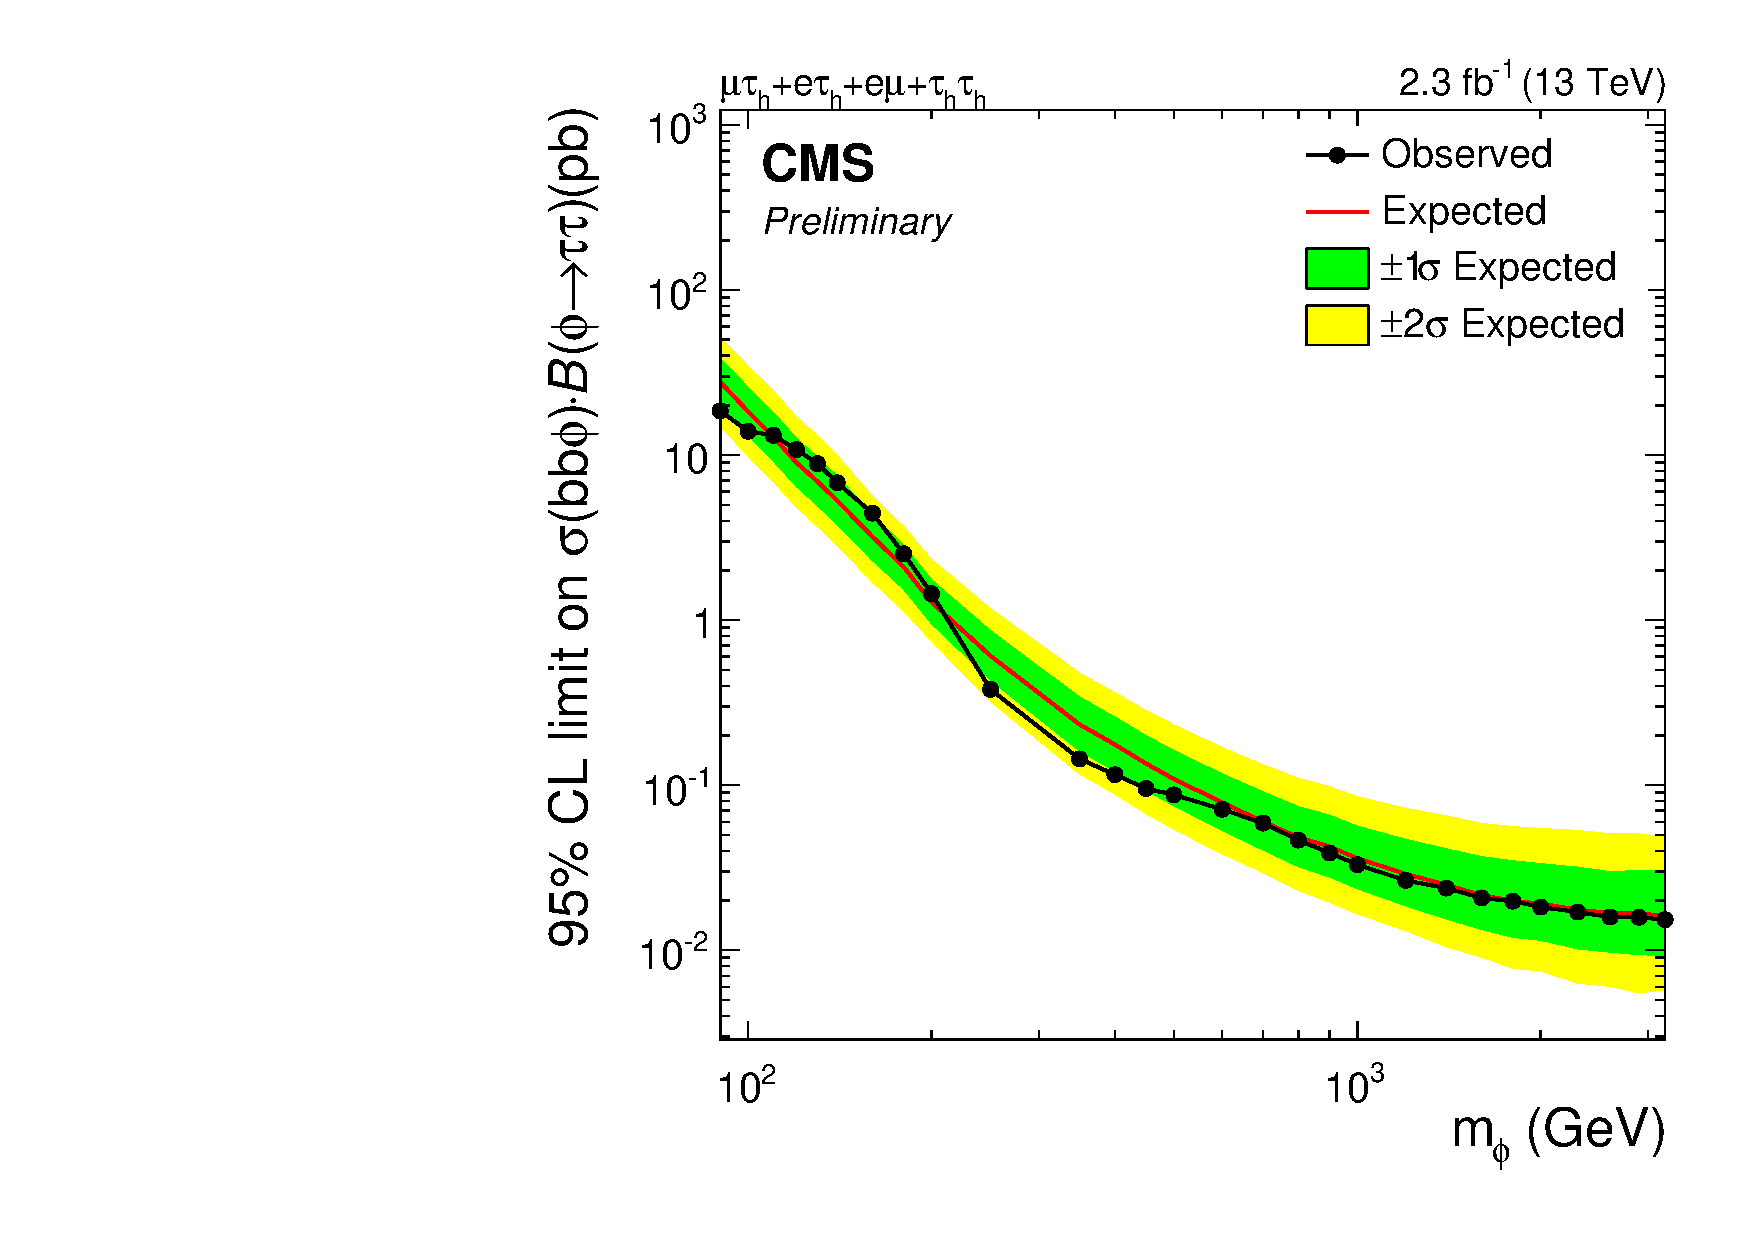
\includegraphics[width=0.48\textwidth, angle=0] {figures/fig_2Htautau_d.pdf}
\caption{ Observed and expected 95\% CL upper limits on the product of cross section and the branching fraction $\sigma(pp\rightarrow \phi) \times B(\phi\rightarrow \tau\tau)$ obtained by the ATLAS collaboration (left) and by the CMS collaboration (right) for the b-associated production.}
\label{fig_2bHtautau}   
\end{figure}

\begin{figure}[tbh!]
\centering
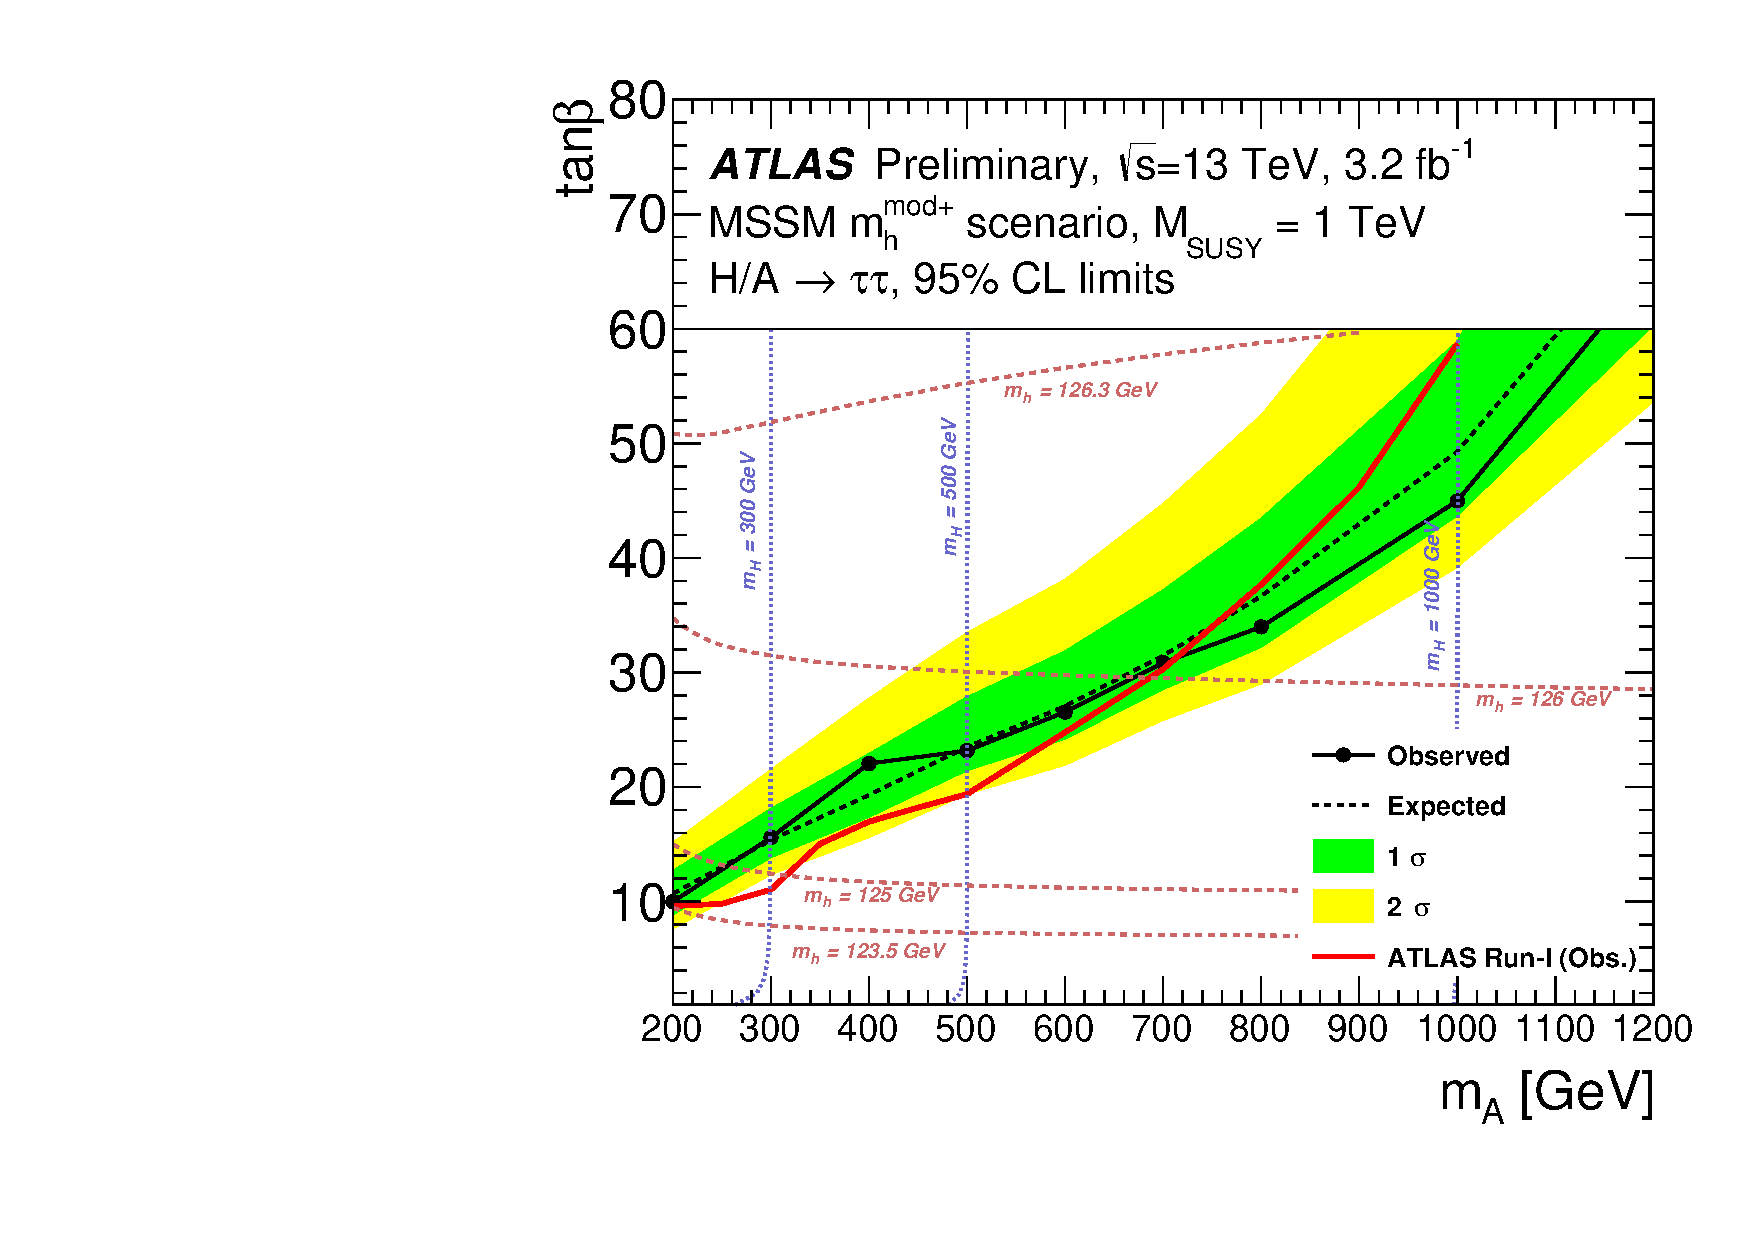
\includegraphics[width=0.48\textwidth, angle=0] {figures/fig_3Htautau_a.pdf}
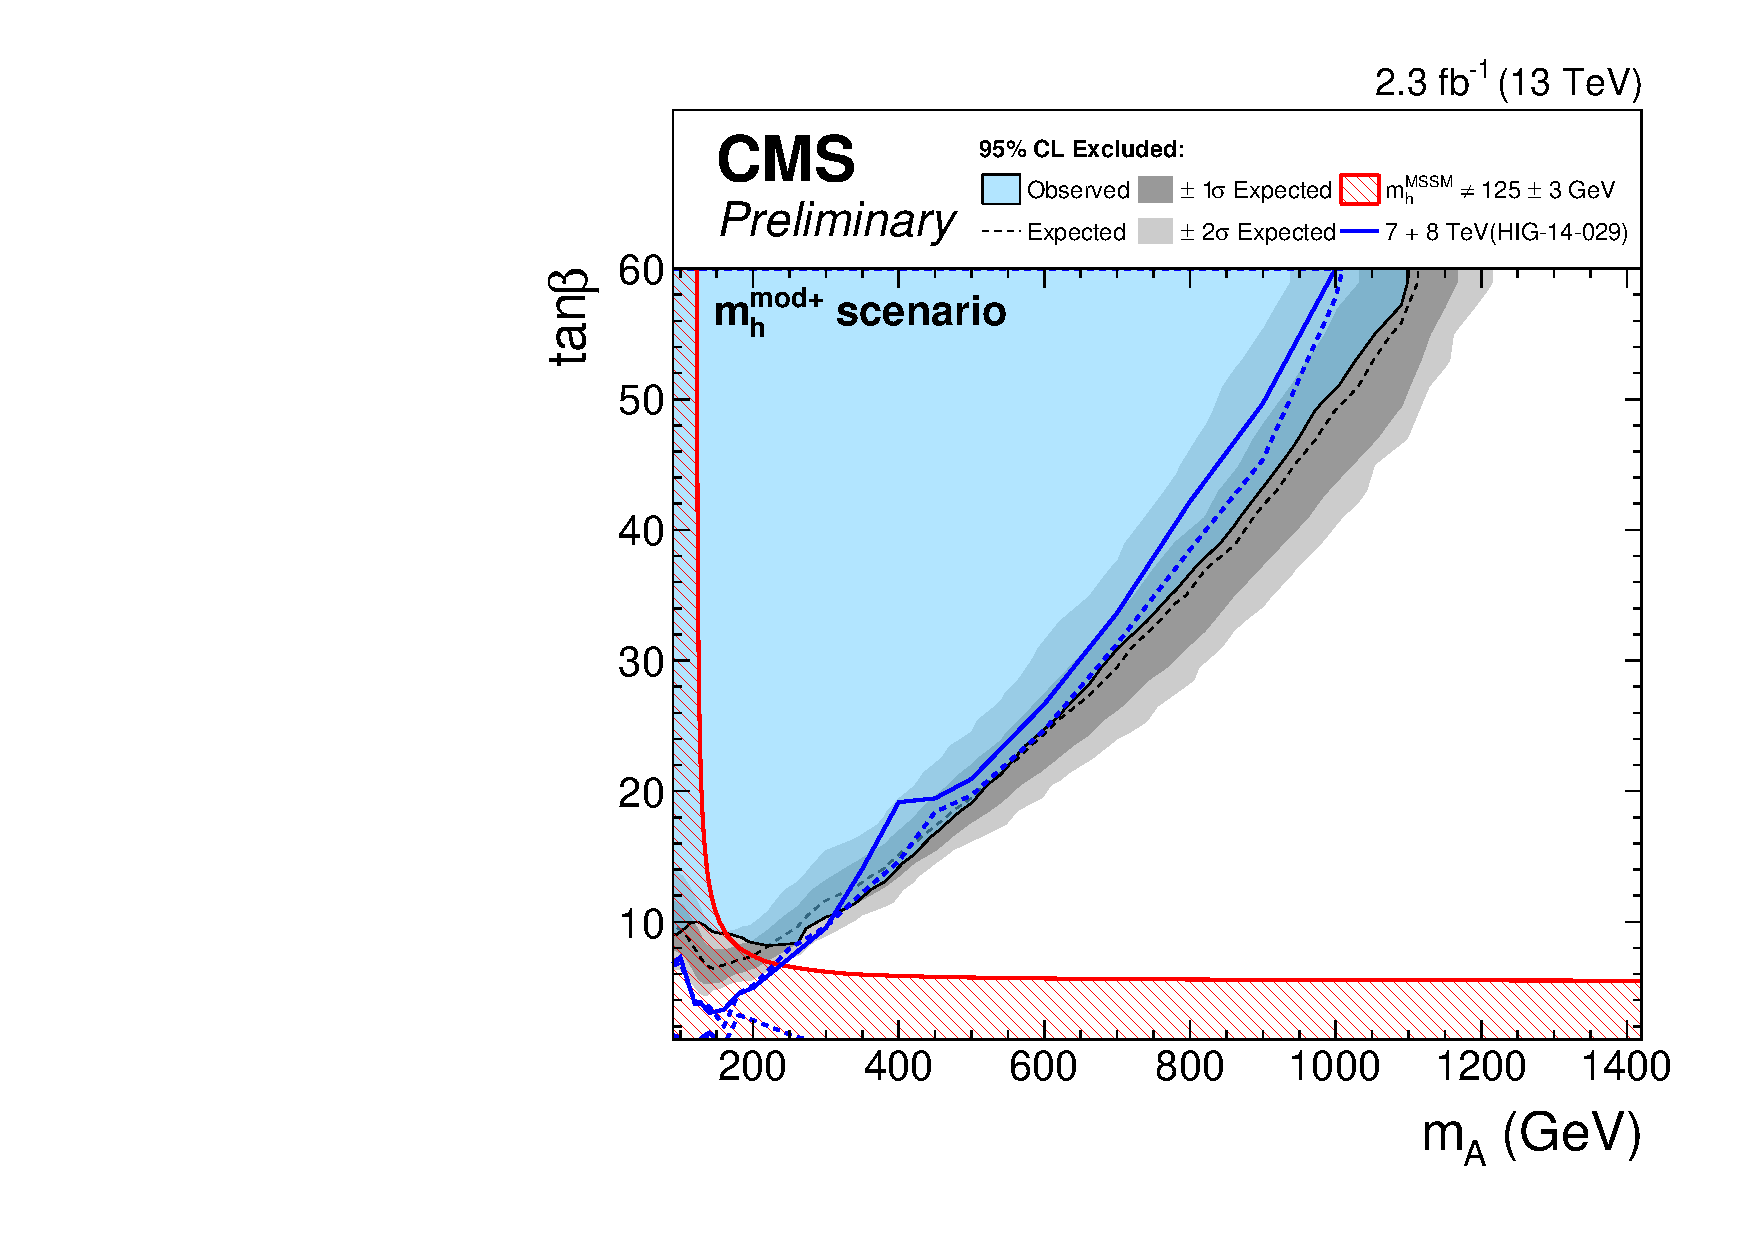
\includegraphics[width=0.48\textwidth, angle=0] {figures/fig_3Htautau_b.pdf}
\caption{ The expected and observed 95\% CL upper limits on tan$\beta$ as a function of $m_{A}$ in the MSSM $m_{h}^{mod+}$ scenario for ATLAS (left) and CMS (right).}
\label{fig_3Htautau}   
\end{figure}

